\documentclass[a4paper,12pt]{article}
\usepackage[utf8]{inputenc}
\usepackage[english]{babel}
\usepackage{graphicx}
\DeclareGraphicsExtensions{.pdf,.png,.jpg}
\usepackage{listings}
\usepackage{hyperref}
\usepackage{float}
\lstset{
language=C,
basicstyle=\footnotesize
}

\title{TDDD56: Lab 2 and 3}
\author{Matteus Hemström (mathe136) and Christian Luckey (chrlu350)}
\begin{document}

\maketitle

\section{Introduction}
This report contains results, answers to questions and conclusions for lab 2 and lab 3. The report is divided into three parts: one section for lab 2 followed by a section for lab 3, and then the last section for our conclusions regarding both labs.

\section{Lab 2}

\begin{itemize}
\item \textit{Write an explaination on how CAS can be used to implement protection for concurrent use of data structures.}

  Compare And Swap (CAS) can be used to implement a lock free concurrent stack by, for example:

  A stack has a head pointer and back pointer. A list item has a next pointer and previous pointer. When we insert an item new\_item into the stack we read the head pointer into last\_item and do a CAS on list.head-$\rangle$next; if head-$\rangle$next == null, swap in new\_item. Next we do a CAS on head pointer; if list.head == last\_item, swap in new\_item.

\item \textit{Sketch a scenario featuring several threads raising the ABA problem.}

Two threads, thread A and thread B are operating on a stack with values 1, 2 and 3. Thread A pop item 1 from the stack, but is interupted just before the CAS. Thread B pops twice getting items 1 and 2, then proceeds by pushing back item 1 onto the stack and frees memory for item 2. When thread A continues with CAS and it will succeed because item 1 is still the stack head. The problem is that the next pointer on item 1 will be pointing to released memory.

\begin{minipage}{\textwidth}
\item \textit{Measure and plot the performance.}

\begin{figure}[H]
  \centering
  \includegraphics[width=0.9\textwidth]{stack_global_timing_both.png}
  \caption{Graph laying it all bare.}
  \label{fig:stacktiming}
\end{figure}

Figure ~\ref{fig:stacktiming} shows that synchronization using hardware CAS is faster than software locks. The performance of the software lock synchronization seems to be harder to predict because it is faster on three threads than two. With the performance test result we can conclude that hardware CAS is preferable. 

\end{minipage}

\item \textit{Explain how CAS can implement a safe data structure sharing between several threads}

By making sure that no one has been changing the stack while we were operating on it we can, sort of, make sure that the CAS stack is a thread safe data structure. If someone has modified the stack, we try again, over and over until we succeed in modifying the stack without anyone else getting between our non-atomic operations.

\begin{minipage}{\textwidth}
\item \textit{Execute a multi-threaded implementation of the test\_aba() unit test}

We implemented test\_aba() by first pushing items with value 1 to the stack. We then proceed by starting three threads that executes the following instructions:

\begin{enumerate}
	\item a = pop()
	\item b = pop()
	\item free(b)
	\item push(a)
\end{enumerate}

We can then detect the ABA-problem by checking the popped values a and b. If any of them does not have value 1, it is because the thread received released memory (as an effect due to the free operation).

During the execution of aba\_test() when the ABA\-problem occurs we get the following output:

\begin{lstlisting})
Aba detected: expected value 1 but received  10798208
\end{lstlisting}

This is an indication that the a pop\-operation received a item which memory has been released.

\end{minipage}
\end{itemize}

\section{Lab 3}

\subsection{Parallel Algorithm Implementation}

	We chose to implement paralell quick sort. The parallelization is done by utilizing new threads for the recursive calls. When executing the recurive quicksort calls the algorithm checks if additional threads are available. If we have an uneven number of threads available we split the work up equally unevenly. That is, we adjust the pivot index to balance the workload over the threads. 

\begin{minipage}{\textwidth}
	There are limitations for our parallel implementation. We do a lot of perhaps unnecessary sorting in order to get a good pivot. But it is important to get a good pivot since it determines the workload balance between the threads.

  \begin{lstlisting}
	if (right - left > 100) {
		int size = (right - left) / 100;
		int copy[size];
		std::copy(&array[left], &array[left + size], copy);
		std::sort(copy, copy + size);
		if (threads_available \% 2 == 0)
			pivot = copy[size / 3];
		else
			pivot = copy[size / 2];
	}
  \end{lstlisting}

  Note that we set the pivot to a third when there are an uneven amount of threads available. This makes sure that the algorithm works well on three cores.
\end{minipage}
\subsection{Drake}

	Our main difficulties with Drake was the lacking documentation. While some documentation did exist, it was hard to get a overview of Drake. The only documentation on Pelab we could find was in the skeleton code, when that documentation was insufficient we had to read the source code of Pelab. We found that it was diffucult to work with Drake because it only worked on computers on ISY or IDA, we could not use our own computers.

	We had the right idea of implementation from the beginning, but we had one bug which took a lot of time to discover because parallel execution is hard to debug. 

\subsection{Results}

\begin{minipage}{\textwidth}

  When going from one to four threads we get a relative speedup of 332\%. The table below shows all the results from sorting 10 million random integers.

  \begin{tabular}{ |l|r| }
	\hline
	NB\_THREADS & time \\
	\hline
    0 & 3564ms \\
    1 & 2491ms \\
    2 & 1338ms \\
    3 & 963ms \\
    4 & 750ms \\
    5 & 725ms \\
    6 & 571ms \\
    12 & 566ms \\
	\hline
  \end{tabular}

  \vspace{10mm}
  
  The table below is the output from a Freja run.

  \begin{tabular}{ |l|r|r|r| }
	  \hline
	   & Type & NB\_THREADS & Relative speedup \\
	  \hline
	  133 &        Drake  &       2    &    1.83 \\
	  134 &     Parallel  &       2    &    2.72 \\
	  135 &        Drake  &       3    &    2.59 \\
	  136 &     Parallel  &       3    &    3.80 \\
	  137 &        Drake  &       4    &    2.30 \\
	  138 &     Parallel  &       4    &    4.87 \\
	  139 &        Drake  &       5    &    2.83 \\
	  140 &     Parallel  &       5    &    5.09 \\
	  141 &        Drake  &       6    &    2.62 \\
	  142 &     Parallel  &       6    &    6.46 \\
	  143 &        Drake  &  Serial    &    1.00 \\
	  144 &     Parallel  &  Serial    &    1.00 \\
	  \hline
  \end{tabular}

\end{minipage}

\begin{figure}[H]
  \centering
  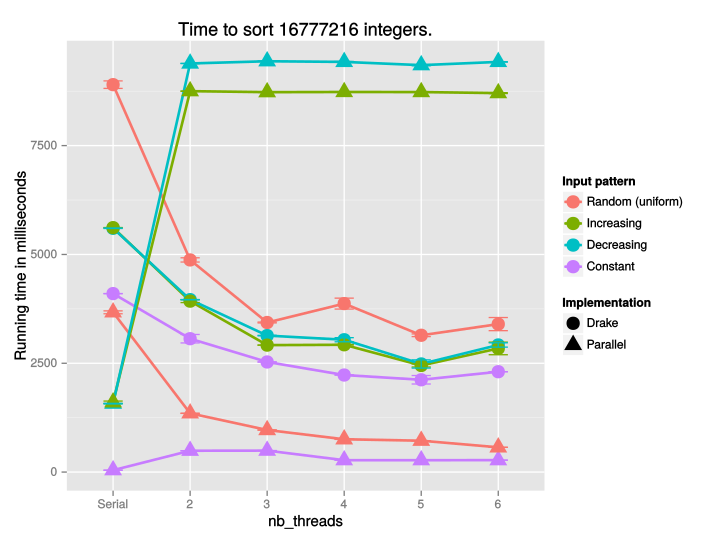
\includegraphics[width=0.9\textwidth]{lab3_time_threads.png}
  \caption{Graph showing execution times on different number of threads.}
  \label{fig:lab3timethreads}
\end{figure}

Figure ~\ref{fig:lab3timethreads} shows that the parallel implementation of quick sort works. The performance of the algorithm is improved when executed on more threads. 


\section{Conclusion}
With the results of lab 2 we conclude that the Compare and Swap (CAS) operation is to prefer over software locks for performance reason. We did however find it easier to work with software locks. Therefore CAS is not nessecary the obvious choice since software locks are faster and easier to implement. 

In lab 3 we implemented a parallel sorting algorithm. We found that our implementaion worked as expected. The parallel algorithm is faster than the sequential version, when executed on six threads it sorted 10 million numbers about four times faster than when executed on a single thread.

It is much harder to draw any conclusions from the results of the Drake part. The results of the Drake application does not show any obvious performance improvements. We believe this is because of two reasons. First of we did solve the communication between the tasks with pop and push of pelib, which is slower than copying whole blocks of memory using peekaddr and writeaddr. The other reason is that there may the issues with the schedule or graph. Working with parallelization using a streaming approach required us to think of the design of the program very carefull, which was a good learning experience. 

\end{document}
